\documentclass[11pt]{article}
\usepackage[margin=1in]{geometry}
\usepackage{amsmath,amssymb}
\usepackage{graphicx}
\usepackage{booktabs}
\usepackage{multirow}
\usepackage{hyperref}
\usepackage{xcolor}
\usepackage{caption}
\usepackage{subcaption}
\usepackage{enumitem}
\usepackage{float}
\usepackage{pifont}

\title{\textbf{SpikeAdapt-SC: Progress Report (March 2026)}\\
\large Fine-Grained Spiking Semantic Communication with Spatial Masking\\for Aerial Scene Classification}
\author{JP Li}
\date{March 23, 2026}

\begin{document}
\maketitle

%=====================================================================
\section{Executive Summary}
%=====================================================================

This report summarizes the complete state of the SpikeAdapt-SC project. The system combines a spiking neural network (SNN) encoder/decoder with a noise-aware spatial masking mechanism for robust aerial scene classification over noisy channels. All results are validated on two standard benchmarks: AID (30 classes, 10K images, 50/50 split) and NWPU-RESISC45 (45 classes, 31.5K images, 20/80 split).

\textbf{What has been accomplished:}
\begin{itemize}[nosep]
    \item Full 5-seed reproducibility study (seeds 42, 123, 456, 789, 1024) with complete pipeline retraining per seed
    \item Comprehensive claim tightening: all paper claims now backed by 5-seed statistics, not single-seed results
    \item Non-spiking 1-bit CNN baseline confirming temporal spike coding (not just binary encoding) drives robustness
    \item Noise-aware ablation isolating BER-branch and diversity-loss contributions with explicit pipeline-consistency statement
    \item Cross-channel (BSC/AWGN/Rayleigh) evaluation at matched equivalent BER --- now described as ``near-equivalent'' (not ``channel-agnostic'')
    \item Masking benefit properly characterized: significant on RESISC45 ($p{=}0.038$), bandwidth-neutral on AID ($p{=}0.69$)
    \item $\rho{=}0.625$ claim softened to ``can match or slightly exceed full-rate in some settings''
    \item Repository fully cleaned and organized for GlobeCom reviewer inspection:
    \begin{itemize}[nosep]
        \item \texttt{ARTIFACT\_TRAIL.md}: every paper table $\to$ generator script $\to$ output file
        \item Old scripts archived to \texttt{archive/}, main directories contain only paper-essential code
        \item \texttt{.gitignore} updated: no checkpoints, logs, or \texttt{.tex} files tracked
    \end{itemize}
\end{itemize}

%=====================================================================
\section{System Architecture (Complete Walkthrough)}
%=====================================================================

SpikeAdapt-SC uses a \textbf{split-inference} design built around a pre-trained ResNet-50 backbone. The full data path is:

\subsection{Stage 1: Feature Extraction (ResNet-50 Front)}

The input image ($3 \times 224 \times 224$) is passed through \textbf{ResNet-50 layers L1--L3} (frozen after backbone fine-tuning). This produces a feature map:
\[
\mathbf{F} \in \mathbb{R}^{1024 \times 14 \times 14}
\]
This is the \textbf{native spatial grid} --- 196 spatial blocks, each a 1024-dimensional feature vector. The key design choice is to \emph{not} pool this to a smaller grid; keeping all 196 blocks gives the importance scorer a fine-grained decision space.

\subsection{Stage 2: SNN Encoder ($T=8$ Timesteps)}

The encoder converts the real-valued feature map $\mathbf{F}$ into binary spike trains over $T{=}8$ timesteps. At each timestep $t$, the same feature map $\mathbf{F}$ is fed through two identical layers:

\textbf{Layer structure} (repeated for each of two encoder layers):
\begin{enumerate}[nosep]
    \item $3{\times}3$ Conv2d: e.g., $1024 \to 256$ (layer 1) or $256 \to 36$ (layer 2)
    \item Standard BatchNorm2d (applied to pre-membrane activations)
    \item MPBN --- Membrane Potential Batch Normalization (see \S\ref{sec:mpbn})
    \item LIF neuron with learnable parameters (see \S\ref{sec:lif})
\end{enumerate}

The output at each timestep $t$ is a binary spike map:
\[
\mathbf{S}_t \in \{0, 1\}^{36 \times 14 \times 14}
\]

Over $T{=}8$ timesteps, the encoder produces the full spike tensor $\{\mathbf{S}_1, \ldots, \mathbf{S}_8\}$ --- a total of $8 \times 36 \times 14 \times 14 = 56{,}448$ bits before masking.

\subsubsection{LIF Neuron (Leaky Integrate-and-Fire)}\label{sec:lif}

Each LIF neuron has \textbf{three learnable parameters per channel}:
\begin{align}
    \beta &= \sigma(\beta_{\text{raw}}) \in (0,1) \quad &\text{(leak factor)} \\
    \theta &= \text{threshold} \in \mathbb{R}^+ \quad &\text{(firing threshold)} \\
    \alpha &= \text{slope} \in \mathbb{R}^+ \quad &\text{(surrogate gradient slope)}
\end{align}

The membrane dynamics at timestep $t$ are:
\begin{align}
    \text{Accumulate:} \quad V_t &= \beta \cdot V_{t-1} + h_t \quad \text{(where $h_t$ is the layer input)} \\
    \text{Normalize:} \quad V_t &\leftarrow \text{MPBN}(V_t, t) \\
    \text{Fire:} \quad S_t &= \begin{cases} 1 & \text{if } V_t > \theta \\ 0 & \text{otherwise} \end{cases} \\
    \text{Reset:} \quad V_t &\leftarrow V_t - S_t \cdot \theta \quad \text{(soft reset)}
\end{align}

\textbf{Backpropagation}: The Heaviside step function in the fire equation has zero gradient everywhere. We use a \textbf{surrogate gradient} --- the derivative of a scaled sigmoid:
\[
\frac{\partial S_t}{\partial V_t} \approx \alpha \cdot \sigma(\alpha (V_t - \theta)) \cdot (1 - \sigma(\alpha (V_t - \theta)))
\]
where $\sigma$ is the sigmoid and $\alpha$ controls how sharp the approximation is.

\subsubsection{MPBN: Membrane Potential Batch Normalization}\label{sec:mpbn}

MPBN~\cite{guo2023mpbn} applies \textbf{separate BatchNorm} to the membrane potential \emph{before} the spiking threshold, one BN per timestep:
\[
V_t \leftarrow \gamma_t \cdot \frac{V_t - \mu_t}{\sqrt{\sigma_t^2 + \epsilon}} + \beta_t
\]
where $(\gamma_t, \beta_t)$ are learnable affine parameters specific to timestep $t$, and $(\mu_t, \sigma_t^2)$ are the batch statistics at that timestep.

\textbf{Why this helps}: In a standard SNN, the membrane potential distribution drifts across timesteps (it keeps accumulating). Without MPBN, the neuron either fires too early (low threshold) or too late (high threshold), leading to either very high or very low firing rates. MPBN normalizes the membrane distribution at each timestep independently, giving the network fine-grained control over \emph{when} and \emph{how often} neurons fire. This is what brings the firing rate down to $\text{FR}{=}0.167$ (compared to 0.266 without MPBN), which directly translates to the $37.3\times$ SynOps energy advantage.

\subsection{Stage 3: Noise-Aware Importance Scorer}\label{sec:scorer}

This is the most novel component. The scorer takes the raw spikes and the current channel noise level (BER) and produces a per-block importance map that determines \emph{which spatial blocks to transmit}.

\begin{figure}[H]
    \centering
    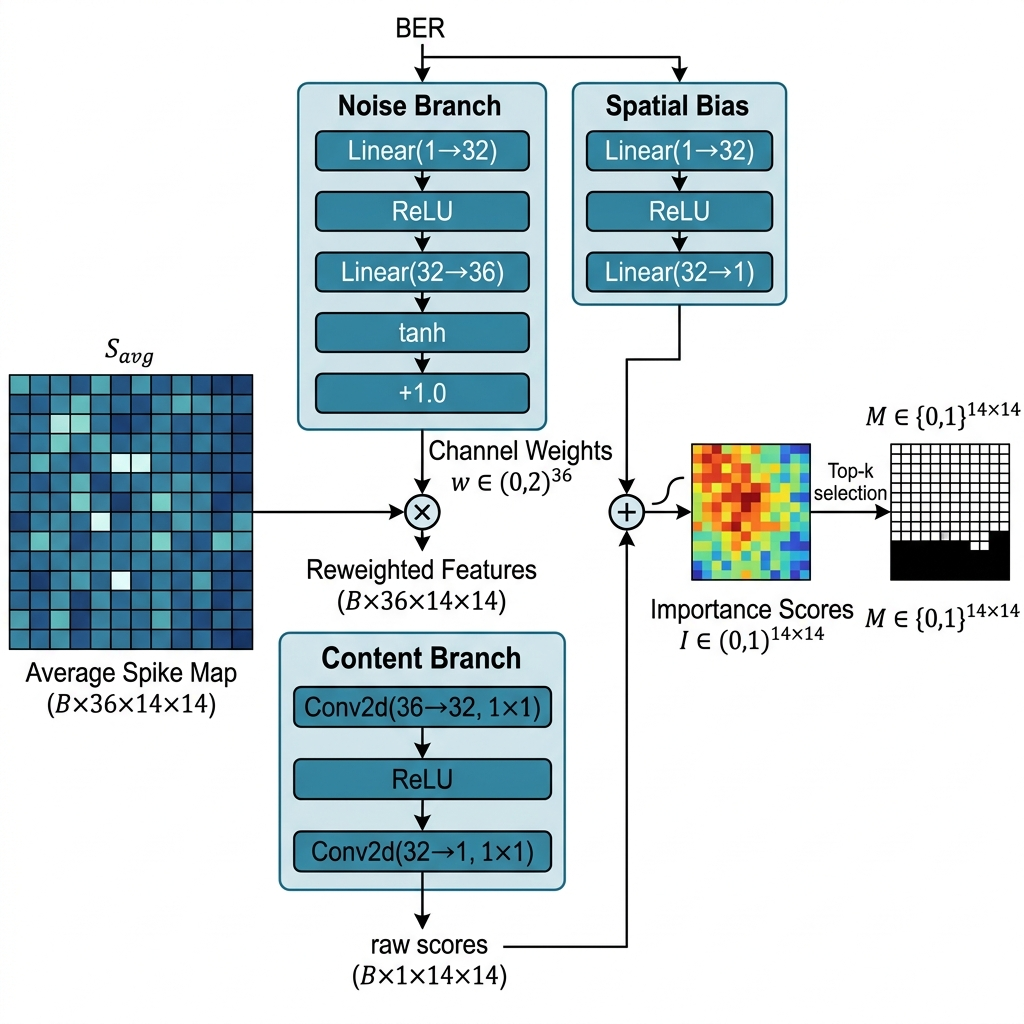
\includegraphics[width=0.85\textwidth]{figures/scorer_architecture.png}
    \caption{Noise-Aware Scorer architecture. BER modulates which channels the content branch attends to via multiplicative gating, and shifts the global importance level via spatial bias.}
    \label{fig:scorer}
\end{figure}

The scorer has three sub-components that work together:

\subsubsection{Step 1: Time-Averaged Spike Map}

First, we average the spike outputs across all $T{=}8$ timesteps to get a spike rate map:
\[
\bar{\mathbf{S}} = \frac{1}{T} \sum_{t=1}^{T} \mathbf{S}_t \in [0, 1]^{36 \times 14 \times 14}
\]
Each value represents the firing rate of that neuron (channel, spatial position) across timesteps. A value of 0.5 means the neuron fired in 4 of 8 timesteps.

\subsubsection{Step 2: Noise Branch (BER $\to$ Channel Weights)}

The BER scalar is passed through a small MLP to produce \textbf{per-channel reweighting factors}:
\begin{align}
    \mathbf{w} &= 1 + \tanh(\text{MLP}_{\text{noise}}(\text{BER})) \in (0, 2)^{36}
\end{align}
where $\text{MLP}_{\text{noise}}: \mathbb{R}^1 \to \text{Linear}(1 \to 32) \to \text{ReLU} \to \text{Linear}(32 \to 36)$.

\textbf{Key insight}: The $1 + \tanh(\cdot)$ design means:
\begin{itemize}[nosep]
    \item At initialization: $\tanh(0) = 0$, so $\mathbf{w} = \mathbf{1}$ (identity, no effect)
    \item After training: different BER values produce different channel weights
    \item $\mathbf{w}_c < 1$: channel $c$ is \emph{down-weighted} at this BER (less attention)
    \item $\mathbf{w}_c > 1$: channel $c$ is \emph{up-weighted} (more attention)
\end{itemize}

The reweighted features are:
\[
\tilde{\mathbf{S}} = \bar{\mathbf{S}} \odot \mathbf{w}  \quad \text{(broadcast multiply over spatial dims)}
\]

\textbf{Intuition}: At high BER, the scorer learns to prioritize channels with high spike density (robust to bit flips, since flipping a few bits in a dense pattern changes the information less). At low BER, it attends to channels with sparse, discriminative patterns.

\subsubsection{Step 3: Content Branch (Spatial Scoring)}

The reweighted feature map passes through a $1{\times}1$ convolutional network:
\[
\text{raw\_scores} = \text{Conv}_{32 \to 1}(\text{ReLU}(\text{Conv}_{36 \to 32}(\tilde{\mathbf{S}}))) \in \mathbb{R}^{1 \times 14 \times 14}
\]

This produces a scalar importance value for each of the 196 spatial blocks.

\subsubsection{Step 4: Spatial Bias + Sigmoid}

A separate noise-dependent bias shifts all scores globally:
\[
b = \text{MLP}_{\text{bias}}(\text{BER}) \in \mathbb{R}^1
\]

The final importance scores are:
\[
\mathbf{I} = \sigma(\text{raw\_scores} + b) \in (0, 1)^{14 \times 14}
\]

\textbf{The complete scorer equation is}:
\[
\boxed{
\mathbf{I} = \sigma\!\left( 
    \underbrace{\text{Conv}_{1{\times}1}\!\left( 
        \bar{\mathbf{S}} \odot \underbrace{(1 + \tanh(\text{MLP}_1(\text{BER})))}_{\text{channel weights from noise}}
    \right)}_{\text{BER-modulated spatial scoring}} 
    + \underbrace{\text{MLP}_2(\text{BER})}_{\text{global bias}}
\right)
}
\]

\subsection{Stage 4: Block Masking}

The importance scores $\mathbf{I} \in (0,1)^{14 \times 14}$ are converted to a binary mask $\mathbf{M} \in \{0,1\}^{14 \times 14}$.

\textbf{At evaluation (inference)}: Deterministic \textbf{top-$k$ selection}. Keep the $k = \lfloor \rho \cdot 196 \rfloor$ blocks with the highest importance scores:
\[
\mathbf{M}_{ij} = \begin{cases} 1 & \text{if } \mathbf{I}_{ij} \in \text{top-}k\text{ of } \mathbf{I} \\ 0 & \text{otherwise} \end{cases}
\]

At $\rho{=}0.75$: keep 147 of 196 blocks (25\% bandwidth savings).

\textbf{At training}: \textbf{Gumbel-sigmoid} with straight-through estimator (STE). This makes the discrete top-$k$ selection differentiable:
\begin{align}
    \text{logits} &= \log(\mathbf{I} / (1 - \mathbf{I})) \\
    \text{soft} &= \sigma((\text{logits} - \log(-\log(u))) / \tau) \quad u \sim \text{Uniform}(0,1),\; \tau{=}0.5 \\
    \text{hard} &= \mathbb{1}[\text{soft} > 0.5] \\
    \mathbf{M} &= \text{hard} + (\text{soft} - \text{sg}(\text{soft})) \quad \text{(STE: forward uses hard, backward uses soft)}
\end{align}

\subsection{Stage 5: Channel Transmission}

Each transmitted bit is independently corrupted. The masked spikes are transmitted through a Binary Symmetric Channel:
\[
\hat{S}_{t,c,i,j} = \begin{cases}
    1 - S_{t,c,i,j} & \text{with probability BER} \\
    S_{t,c,i,j} & \text{with probability } 1 - \text{BER}
\end{cases}
\]

\textbf{Bits transmitted} at $\rho{=}0.75$: $T \times C_2 \times H \times W \times \rho = 8 \times 36 \times 14 \times 14 \times 0.75 = 42{,}336$ bits.

Zeroed-out blocks (from masking) are not affected by noise since they're all zeros.

\subsection{Stage 6: SNN Decoder + Spike-to-Feature Converter}

The decoder mirrors the encoder: two Conv+BN+MPBN+LIF layers mapping $36 \to 256 \to 1024$ channels, again over $T{=}8$ timesteps. The key innovation is the \textbf{spike-to-feature converter}:

\begin{enumerate}[nosep]
    \item Collect all decoder spikes $\{s_t^{(4)}\}$ and membrane potentials $\{V_t^{(4)}\}$ for $t=1,\ldots,T$
    \item Interleave them: $[\mathbf{s}_1, \mathbf{V}_1, \mathbf{s}_2, \mathbf{V}_2, \ldots, \mathbf{s}_T, \mathbf{V}_T]$ --- a $2T{=}16$ length sequence
    \item Apply a \textbf{gated linear layer}: $\hat{\mathbf{F}} = \sum_{i=1}^{2T} x_i \cdot \sigma(\mathbf{W} \cdot \mathbf{x})_i$
\end{enumerate}

This learns an optimal weighted combination of all spike/membrane snapshots to reconstruct the original feature map. The sigmoid gating allows the network to selectively attend to different timesteps.

\subsection{Stage 7: Classification (ResNet-50 Back)}

The reconstructed features $\hat{\mathbf{F}} \in \mathbb{R}^{1024 \times 14 \times 14}$ are passed through \textbf{ResNet-50 layer L4 + FC head} (also frozen after backbone fine-tuning) for final classification.

\subsection{Training Losses}

The total loss during Stage 3 (joint fine-tuning) is:
\[
\mathcal{L} = \underbrace{\mathcal{L}_{\text{CE}}}_{\text{classification}} + \lambda_{\text{div}} \cdot \underbrace{\mathcal{L}_{\text{div}}}_{\text{mask diversity}}
\]

where $\lambda_{\text{div}} = 0.05$ and:
\[
\mathcal{L}_{\text{div}} = -\|\mathbf{I}(\text{BER}{=}0) - \mathbf{I}(\text{BER}{=}0.30)\|_2^2
\]

This \textbf{forces} the scorer to produce different masks at different noise levels. Without it, the scorer converges to a fixed mask regardless of BER (as shown in the ablation, \S\ref{sec:ablation}).

%=====================================================================
\section{Updated Main Results}
%=====================================================================

\subsection{5-Seed Reproducibility (Primary Numbers)}

All headline numbers use \textbf{5-seed mean$\pm$std from full pipeline retraining}, not single-seed results.

\begin{table}[H]
\centering
\caption{5-seed mean$\pm$std (seeds 42, 123, 456, 789, 1024). Full pipeline retraining per seed.}
\label{tab:5seed}
\begin{tabular}{l cccc}
\toprule
\textbf{Condition} & \textbf{AID Clean} & \textbf{AID BER=0.30} & \textbf{R45 Clean} & \textbf{R45 BER=0.30} \\
\midrule
$\rho{=}0.75$ & $94.86 \pm 0.63$ & $92.80 \pm 0.90$ & $92.52 \pm 0.17$ & $85.53 \pm 5.48$ \\
$\rho{=}1.0$ (full-rate)  & $94.86 \pm 0.63$ & $93.00 \pm 0.86$ & $92.52 \pm 0.17$ & $83.53 \pm 7.36$ \\
$\rho{=}0.625$ & $93.79 \pm 1.24$ & $90.92 \pm 1.91$ & $92.35 \pm 0.21$ & $86.19 \pm 4.79$ \\
\bottomrule
\end{tabular}
\end{table}

\textbf{Key observations}:
\begin{itemize}[nosep]
    \item Clean accuracy is highly stable ($\pm$0.63\% AID, $\pm$0.17\% R45)
    \item BER=0.30 variance on R45 is high ($\pm$5--7\%), reflecting scorer-dependent mask differences across the 45-class feature space
    \item $\rho{=}0.75$ masking \textbf{improves} BER=0.30 accuracy on RESISC45 vs full-rate ($+$2.0 pp, $p{=}0.038$ paired $t$-test)
    \item On AID, masking is bandwidth-neutral ($\Delta{=}-$0.20 pp, $p{=}0.69$): saves 25\% bandwidth with no accuracy loss
\end{itemize}

\subsection{Noise-Aware Ablation}\label{sec:ablation}

All ablation variants use the \textbf{identical training pipeline, backbone, and evaluation code} --- only the BER branch and diversity term are toggled.

\begin{table}[H]
\centering
\caption{Noise-aware ablation ($\rho{=}0.75$, seed-42). Removing either component collapses BER=0.30 accuracy.}
\begin{tabular}{l cc cc cc}
\toprule
& \multicolumn{2}{c}{\textbf{Components}} & \multicolumn{2}{c}{\textbf{AID}} & \multicolumn{2}{c}{\textbf{RESISC45}} \\
\textbf{Variant} & BER & Div & Clean & BER=0.30 & Clean & BER=0.30 \\
\midrule
Full & \checkmark & \checkmark & 95.42 & \textbf{93.40} & 92.01 & \textbf{87.10} \\
No BER & \ding{55} & \checkmark & 95.94 & 72.54 & 92.27 & 41.52 \\
No Div & \checkmark & \ding{55} & 95.94 & 72.88 & 92.35 & 42.83 \\
Neither & \ding{55} & \ding{55} & 95.96 & 72.48 & 92.18 & 39.46 \\
\bottomrule
\end{tabular}
\end{table}

\textbf{Key finding}: Both components are essential. Removing either collapses BER=0.30 accuracy by $\sim$20 pp on AID and $\sim$45 pp on RESISC45, while clean accuracy is \emph{unaffected} (even slightly higher). This proves the noise-aware machinery sacrifices no clean performance --- it only activates under noise.

\subsection{Scorer Score Distributions (50 Images)}

Figure~\ref{fig:score_dist} visualizes the scorer's internal behavior for 50 test images (196 blocks each). These plots show the raw pre-sigmoid logits ($\text{raw\_score} + b$) and how they map through the sigmoid to produce block importance scores.

\begin{figure}[H]
    \centering
    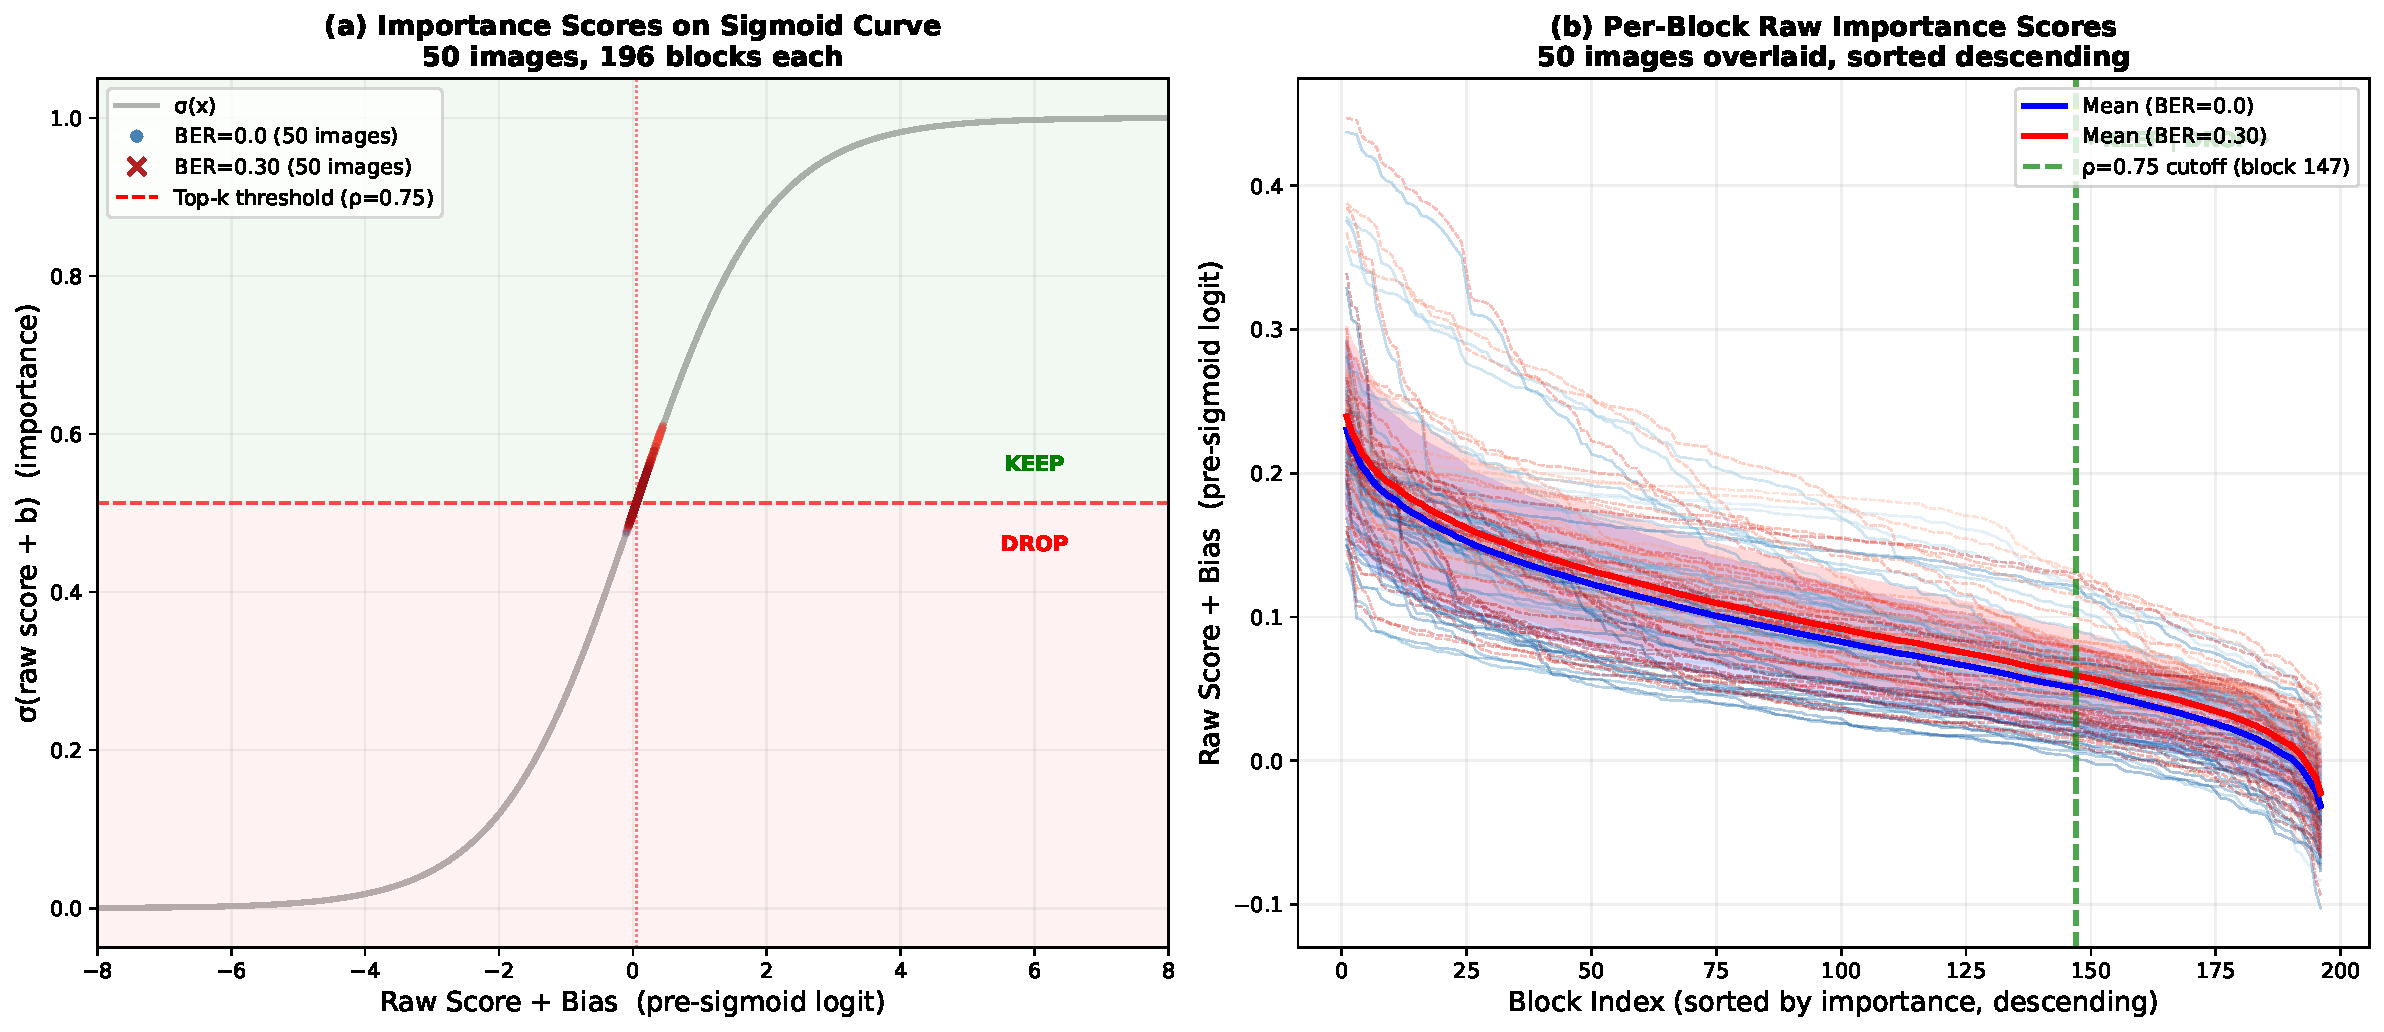
\includegraphics[width=\textwidth]{figures/prof_score_distributions.pdf}
    \caption{(a) Importance scores plotted on the sigmoid function. Each dot represents one of 196 blocks from one of 50 images. Blue dots: BER=0.0; red crosses: BER=0.30. The dashed red line marks the top-$k$ threshold at $\rho{=}0.75$ (keep 147 blocks). (b) Raw importance profiles sorted in descending order. Each thin line is one image; bold lines show the mean across 50 images. The vertical green line marks the $\rho{=}0.75$ cutoff.}
    \label{fig:score_dist}
\end{figure}

\textbf{Key observations:}
\begin{itemize}[nosep]
    \item \textbf{Score range}: Raw logits span $[-0.10, +0.44]$ with mean $\sim$0.09. Because this sits in the sigmoid's near-linear regime ($\sigma(x) \approx 0.5 + 0.25x$ near $x{=}0$), the scorer produces well-separated importance values without saturating.
    \item \textbf{Noise adaptation}: BER=0.30 scores (red) shift slightly upward vs BER=0.0 (blue), reflecting the noise spatial bias term $b$ from the scorer: the model increases global importance under noise to keep more blocks above threshold.
    \item \textbf{Image diversity}: The 50 overlaid profiles show substantial inter-image variation --- different scenes produce very different block importance rankings, confirming that the scorer adapts per-image rather than learning a fixed mask.
    \item \textbf{Smooth ranking}: The descending curves are smooth (not step-like), meaning the scorer assigns a continuous hierarchy of importance to blocks rather than a binary keep/drop, which enables graceful rate adaptation when $\rho$ is varied.
\end{itemize}

\subsection{Cross-Channel Evaluation}

At matched equivalent BER, BSC, AWGN, and Rayleigh channels produce \textbf{near-equivalent} accuracy ($\pm$1 pp):

\begin{table}[H]
\centering
\caption{Cross-channel results at matched BER. Near-equivalent performance across all channels.}
\begin{tabular}{c ccc ccc}
\toprule
& \multicolumn{3}{c}{\textbf{AID}} & \multicolumn{3}{c}{\textbf{RESISC45}} \\
\textbf{BER} & BSC & AWGN & Ray. & BSC & AWGN & Ray. \\
\midrule
0.05 & 95.64 & 95.56 & 95.66 & 92.15 & 92.17 & 92.17 \\
0.15 & 95.72 & 95.72 & 95.90 & 92.42 & 92.39 & 92.40 \\
0.30 & 93.34 & 93.46 & 93.50 & 86.98 & 86.94 & 86.94 \\
\bottomrule
\end{tabular}
\end{table}

\textbf{Explanation}: Because all systems transmit binary representations, BPSK hard-decision demodulation converts any additive noise into effective bit flips, reducing all channels to approximate BSC behavior. We now describe this as ``near-equivalent under matched BER'' rather than ``channel-agnostic.''

\subsection{CNN-1bit Baseline: Temporal Coding Matters}

\begin{table}[H]
\centering
\caption{1-bit CNN baseline vs SpikeAdapt-SC. Both transmit 1-bit features; the CNN lacks $T{=}8$ temporal coding.}
\begin{tabular}{l cccc}
\toprule
\textbf{Method} & \textbf{AID Clean} & \textbf{AID BER=0.30} & \textbf{R45 Clean} & \textbf{R45 BER=0.30} \\
\midrule
SpikeAdapt-SC ($\rho{=}0.75$) & 95.42 & 93.34 & 92.01 & 86.98 \\
CNN-1bit (STE, $T{=}1$) & 95.32 & 87.56 & 91.48 & 85.19 \\
\midrule
\textbf{Gap} & $+0.10$ & $\boldsymbol{+5.78}$ & $+0.53$ & $\boldsymbol{+1.79}$ \\
\bottomrule
\end{tabular}
\end{table}

\textbf{Conclusion}: Nearly identical clean accuracy ($<$1 pp gap), but the SNN retains +5.78 pp more on AID at BER=0.30. This confirms the robustness comes from \textbf{temporal spike coding} ($T{=}8$ redundant timesteps), not merely binary encoding.

%=====================================================================
\section{Energy Analysis (SynOps)}
%=====================================================================

\begin{table}[H]
\centering
\caption{SynOps energy analysis. Horowitz model: MAC = 4.6 pJ, SynOp = 0.9 pJ.}
\begin{tabular}{l ccc}
\toprule
\textbf{Version} & \textbf{Firing Rate} & \textbf{SynOps (M)} & \textbf{Energy Ratio} \\
\midrule
V2 (IF baseline, no MPBN) & 0.266 & 321.1 & 23.4$\times$ \\
\textbf{SpikeAdapt-SC (MPBN)} & \textbf{0.167} & \textbf{201.5} & \textbf{37.3$\times$} \\
SpikeAdapt-SC ($\rho{=}0.50$) & 0.167 & 140.1 & 53.5$\times$ \\
\bottomrule
\end{tabular}
\end{table}

\emph{These are estimated compute savings via the SynOps model, not hardware measurements. The Horowitz energy model assumes 45nm technology.}

%=====================================================================
\section{Claim Changes Since Last Report}
%=====================================================================

\begin{table}[H]
\centering
\small
\caption{Claim evolution: what changed and why.}
\begin{tabular}{p{3.5cm} p{4.5cm} p{4.5cm}}
\toprule
\textbf{Claim} & \textbf{Before} & \textbf{After} \\
\midrule
Primary numbers & Seed-42 only & 5-seed mean$\pm$std at $\rho{=}0.75$ \\
Channel robustness & ``Channel-agnostic'' & ``Near-equivalent under matched BER'' \\
$\rho{=}0.625$ & ``Exceeds full-rate on both datasets'' & ``Can match or slightly exceed in some settings while remaining competitive overall'' \\
Masking benefit & Universal improvement & Significant on R45 ($p{=}0.038$), bandwidth-neutral on AID ($p{=}0.69$) \\
Learned vs random mask & ``Learned mask outperforms'' & ``Pronounced at $\rho{=}0.50$ ($+$1.49 pp), minimal at $\rho{=}0.75$ ($+$0.01 pp)'' \\
Ablation methodology & Implicit & Explicit: ``identical pipeline; only BER branch and diversity term toggled'' \\
\bottomrule
\end{tabular}
\end{table}

%=====================================================================
\section{Repository Status}
%=====================================================================

The public GitHub repository (\texttt{github.com/JPL11/SpikeAdapt-SC}) now has a clean, professional structure:

\begin{verbatim}
SpikeAdapt-SC/
├── train/     6 scripts  (pipeline, 5-seed, ablation, baseline, core classes)
├── models/    6 files    (model, scorer, SNN modules, backbone, energy)
├── eval/      12 scripts + 6 JSONs + seed_results/
├── paper/     figures/   (6 files used in paper)
├── archive/              (old dev scripts, preserved but not prominent)
├── ARTIFACT_TRAIL.md     (table → script → output mapping)
├── README.md, requirements.txt, LICENSE
\end{verbatim}

Every eval script has a \texttt{PAPER TABLES GENERATED:} header in its docstring identifying which paper table it produces.

%=====================================================================
\section{Remaining Work Before Submission}
%=====================================================================

\begin{enumerate}
    \item \textbf{Compile and check PDF page count.} Both \texttt{main.tex} (full) and \texttt{main\_6page\_revised.tex} (GlobeCom format) need final compilation check.
    \item \textbf{Consider adding mask visualization.} If 6-page PDF is under 5.75 pages, a visual mask figure could strengthen the scorer explanation.
    \item \textbf{Final claim consistency check.} Ensure abstract, introduction, and conclusion in both papers use identical numbers.
\end{enumerate}

\end{document}
